\documentclass[11pt]{article}
    
% =================================================================================================================================================================================== %
%%%%%%%%%%%%%%%%%%%%%%%%%%%%%%%%%%%%%%%%%%%%%%%%%%%%%%%%%%%%%%%%%%%%%% ----- Préambule : gestion des librairies ----- %%%%%%%%%%%%%%%%%%%%%%%%%%%%%%%%%%%%%%%%%%%%%%%%%%%%%%%%%%%%%%%%%
% =================================================================================================================================================================================== %

\usepackage[a4paper, margin=2.5cm]{geometry} % Marges de 2.5 cm de chaque côté
\usepackage{wrapfig}
\usepackage[french]{babel} % Utilisation de la langue française
\usepackage[utf8]{inputenc} % Gestion des accents / encodage des fichiers utf8 (alternative latin1)
\usepackage[T1]{fontenc}
\usepackage{lmodern}
\usepackage{graphicx} % Insertion des illustrations
\usepackage{xcolor} % Colorisation syntaxique
\definecolor{sectioncolor}{HTML}{880E4F}
\definecolor{subsectioncolor}{HTML}{BF360C}
\usepackage[colorlinks = TRUE]{hyperref}
\usepackage{array}
\usepackage{float}
\usepackage{tcolorbox}

\usepackage{graphicx}
\usepackage{xcolor}
\usepackage[colorlinks = TRUE]{hyperref}
\usepackage{array}

\usepackage{anyfontsize}
\usepackage{caption}
\DeclareCaptionLabelFormat{custom}{#1 #2\hspace{0.5ex}}
\DeclareCaptionLabelSeparator{custom}{ - \hspace{0.5ex}}
\DeclareCaptionFormat{custom}{#1#2 #3}
\captionsetup[figure]{labelformat = custom,
                      labelsep = custom,
                      format = custom,
                      name = Fig.}

\usepackage{tocloft}
\def\frenchcontentsname{\bfseries \fontsize{17}{17} \selectfont Sommaire \vspace{0.3cm}}  
\renewcommand{\cfttoctitlefont}{\hspace{6.5cm} \normalsize \MakeUppercase}
\setcounter{secnumdepth}{2} 
\makeatletter
\renewcommand{\cftsecleader}{\cftdotfill{\cftdotsep}}
\makeatother
\hypersetup{colorlinks = true,linkcolor = blue} 
\setlength\cftaftertoctitleskip{0.1cm}
\renewcommand{\cftbeforesecskip}{7pt}
\renewcommand{\cftsecafterpnum}{\vskip3pt}
\renewcommand{\cftsubsecafterpnum}{\vskip3pt}
\renewcommand{\cftsecfont}{\sffamily \bfseries \large}
\renewcommand{\cftsubsecfont}{\sffamily \normalsize}

\usepackage{titlesec}
\usepackage{setspace}
\titleformat{\section}{\fontsize{16}{15}\bfseries \color{sectioncolor}}{\thesection \hspace{0.2cm}-}{0.2cm}{}
\titlespacing{\section}{0.3cm}{0.5cm}{0.2cm}
\titleformat{\subsection}{\fontsize{14}{15}\bfseries \color{subsectioncolor}}{\thesubsection}{0.2cm}{}
\titlespacing{\subsection}{0.6cm}{0.5cm}{0.2cm}

% =================================================================================================================================================================================== %
%%%%%%%%%%%%%%%%%%%%%%%%%%%%%%%%%%%%%%%%%%%%%%%%%%%%%%%%%%%%%%%%%%%%%%%%%%%%%%% ----- Début du document ----- %%%%%%%%%%%%%%%%%%%%%%%%%%%%%%%%%%%%%%%%%%%%%%%%%%%%%%%%%%%%%%%%%%%%%%%%%
% =================================================================================================================================================================================== %

\begin{document}

\pagenumbering{arabic}
\thispagestyle{empty}

%% --- Page de couverture --- %%

\begin{tabular}{m{0.2\textwidth}m{0.48\textwidth}m{0.1\textwidth} }
\includegraphics[scale=0.65]{Images/logo-univ} & \centering {\fontsize{22}{15}\selectfont \bf Université de Caen \\[0.3cm] Normandie}  & \includegraphics[scale=0.50]{Images/logo-iut}
\end{tabular}

\vspace{1cm}

\begin{center}
{\fontsize{24}{15}\selectfont IUT Grand Ouest Normandie}

\vspace{0.5cm}

{\LARGE Pôle de Caen}

\vspace{1.cm}

{\fontsize{20}{15}\selectfont Bachelor Universitaire de Technologie}

\vspace{0.4cm}

{\fontsize{20}{15}\selectfont \bf Science des Données}

\vspace{1.25cm}

{\Large \tt Deuxième année}

\vspace{0.3cm}

{\Large Ressource : Développement d’un composant d’une solution décisionnelle}

\vspace{1cm}

\rule{0.5\textwidth}{1pt}

\vspace{0.8cm}

{\fontsize{20}{15}\selectfont \textcolor{purple}{\bf Tableau de Bord Interactif pour l'Analyse de l'Économie Mondiale}}

\vspace{1cm}

\includegraphics[scale=0.4]{Images/image-titre.png}

\vspace{0.3cm}
 
\rule{0.5\textwidth}{1pt}

\vspace{0.3cm}

{\Large \bf Auteurs}

\vspace{0.1cm}

{\tt Romain LESUEUR}\\[0.2cm]
{\tt Anthony YON}\\[0.2cm]
{\tt Mandir DIOP}\\[0.2cm]
{\tt Courteney SAINT-HUBERT}

\vspace{1.7cm}

{\large Année universitaire 2024-2025}

\end{center}

%%%%%%%%%%%%%%%%%
\pagebreak
%%%%%%%%%%%%%%%%%

\vspace*{1cm}
\tableofcontents

%%%%%%%%%%%%%%%%%
\pagebreak
%%%%%%%%%%%%%%%%%

\section*{\begin{center} \Huge Introduction \end{center}}
\addcontentsline{toc}{section}{\Large Introduction \vspace{0.3cm}}

\subsection*{Présentation du projet}

Ce projet a pour objectif de concevoir un outil interactif et intuitif permettant de visualiser et d'analyser des données économiques mondiales. Dans un contexte où les données économiques jouent un rôle crucial dans la prise de décisions stratégiques, ce tableau de bord vise à offrir une vue d'ensemble des principaux indicateurs économiques tels que le PIB, la croissance démographique, l'espérance de vie, le développement humain, et la consommation énergétique.

L'idée principale est de transformer des données complexes en visualisations claires et accessibles, facilitant ainsi la compréhension des grandes tendances économiques mondiales. Grâce à des graphiques dynamiques et une carte interactive, les utilisateurs peuvent explorer les données par région, par pays, ou encore par période, tout en mettant en lumière les disparités régionales et les opportunités de développement.

Ce projet ne se limite pas à une simple présentation des données. Il s'agit également d'un exercice technique et collaboratif, mobilisant des compétences en développement web, en gestion de base de données, et en visualisation de données. En combinant des technologies modernes comme Chart.js et D3.js, nous avons cherché à créer un outil performant, ergonomique, et adapté aux besoins des utilisateurs.

En somme, ce tableau de bord interactif se veut être un outil pédagogique et analytique, permettant à la fois de mieux comprendre les dynamiques économiques globales et de valoriser les compétences techniques acquises au cours de cette formation.

\subsection*{Stack technique imposée}
Le projet utilise les technologies suivantes :
\begin{itemize}
  \item \textbf{Frontend} : HTML, CSS, JavaScript (Chart.js pour les visualisations, D3.js pour la carte interactive)
  \item \textbf{Backend} : PHP
  \item \textbf{Base de données} : MySQL (gérée via phpMyAdmin avec XAMPP)
  \item \textbf{Outils de versionnement} : Git + GitHub
\end{itemize}

En outre, une contrainte importante était d'utiliser une structure basée sur le modèle MVC (Modèle-Vue-Contrôleur) pour organiser le projet. Cette approche a permis de séparer clairement la logique métier (modèle), la gestion des interactions utilisateur (contrôleur), et l'affichage des données (vue). Une autre contrainte imposée était de ne pas utiliser de classes, ce qui nous a poussés à structurer le code en utilisant des fonctions et des fichiers bien organisés pour maintenir la lisibilité et la modularité.

\newpage

\subsection*{Répartition des tâches initiales et méthodologie de travail}
\begin{itemize}
  \item \textbf{Anthony YON} :
    \begin{itemize}
      \item Création et maintien du code dans \texttt{\detokenize{/models/pays.php}}.
      \item Création et maintien du code dans \texttt{\detokenize{/views/dashboard.php}}.
      \item Product Owner de la partie \texttt{\detokenize{/controllers/indicateurs.php}} concernant le dashboard principal.
      \item Création et maintien du code concernant les headers/footers.
      \item Création d'au moins un graphique sur le dashboard principal.
    \end{itemize}
  \item \textbf{Mandir DIOP} :
    \begin{itemize}
      \item Création et maintien du code dans \texttt{\detokenize{config.inc.php}}.
      \item Création et maintien du code dans \texttt{\detokenize{/models/indicateur.php}}.
      \item Création du MLD (Modèle Logique de Données).
      \item Création et maintien du code dans \texttt{\detokenize{/views/infos_pays.php}}.
            \item Création et maintien du code dans \texttt{\detokenize{/controllers/indicateur.php}} \par concernant \texttt{\detokenize{/views/infos_pays.php}}.
      \item Création d'au moins un graphique sur le dashboard principal.
    \end{itemize}
  \item \textbf{Romain LESUEUR} :
    \begin{itemize}
      \item Création et maintien du code dans \texttt{\detokenize{/models/data.php}}.
      \item Création et maintien du dossier \texttt{\detokenize{/tests/}}.
      \item Création et maintien du logger.
      \item Assistance sur le développement des parties \texttt{\detokenize{/views/}} et \texttt{\detokenize{/controllers/}}.
           \item Création et maintien du code dans \texttt{\detokenize{/controllers/indicateurs.php}} concernant le dashboard principal.
      \item Création et maintien des fichiers suivants : \texttt{\detokenize{DEV.md}}, \texttt{\detokenize{README.md}}, \texttt{\detokenize{.htaccess}}, \texttt{\detokenize{/docs/howtogit.md}}.
      \item Création d'au moins un graphique sur le dashboard principal.
      \item Supervision de tout le projet.
    \end{itemize}
  \item \textbf{Courteney SAINT-HUBERT} :
    \begin{itemize}
      \item Création et maintien du code dans \texttt{\detokenize{/models/indices.php}}.
      \item Création du MCD (Modèle Conceptuel de Données).
      \item Création et maintien du code dans \texttt{\detokenize{/views/comparaison_pays.php}}.
      \item Création et maintien du code dans \texttt{\detokenize{/controllers/indicateurs.php}} \par concernant \texttt{\detokenize{/views/comparaison_pays.php}}.
      \item Création d'au moins un graphique sur le dashboard principal.
    \end{itemize}
\end{itemize}

En outre, le projet a été versionné sur GitHub, ce qui a grandement facilité la gestion collaborative et le suivi des modifications. Vous pouvez consulter le dépôt GitHub à l'adresse suivante : 
\href{https://github.com/EkiaND/DED}{https://github.com/EkiaND/DED}.

En tant que superviseur du projet (Romain), j'ai joué un rôle central dans la coordination et la validation des tâches. À chaque push, je réalisais une revue du code pour vérifier sa qualité et sa fonctionnalité. Si le code était fonctionnel, nous discutions ensemble des éventuelles améliorations possibles. En cas d'erreurs, je les expliquais en détail à l'auteur, que ce soit des erreurs logiques ou de code, souvent lors d'appels pour clarifier les points complexes. Ce processus a permis d'assurer une progression continue et une amélioration constante de la qualité du projet.


%%%%%%%%%%%%%%%%%
\pagebreak
%%%%%%%%%%%%%%%%%

\section{Contexte et Objectifs}

\subsection{Contexte du projet}

Dans un monde où l’économie évolue rapidement, les données économiques jouent un rôle crucial dans la compréhension des dynamiques globales et la prise de décisions stratégiques. Chaque jour, une quantité massive de données est produite, couvrant des aspects variés tels que la croissance démographique, le PIB, l'espérance de vie, ou encore la consommation énergétique. Cependant, ces données, bien que riches en informations, restent souvent complexes et difficiles à interpréter sans outils adaptés.

C'est dans ce contexte que la nécessité de développer des outils de visualisation clairs, interactifs et informatifs se fait sentir. Ces outils permettent de transformer des données brutes en informations exploitables, facilitant ainsi l'analyse et la compréhension des grandes tendances économiques mondiales. Ils offrent également la possibilité de mettre en lumière les disparités régionales, les opportunités de développement, et les relations entre différents indicateurs économiques.

En outre, l'évolution rapide des technologies numériques a ouvert de nouvelles perspectives pour la visualisation de données. Les outils modernes permettent désormais de créer des interfaces interactives et dynamiques, rendant les analyses plus accessibles et engageantes pour les utilisateurs. Ce projet s'inscrit dans cette dynamique, en cherchant à répondre aux besoins croissants d'analyse économique dans un monde de plus en plus interconnecté.

\subsection{Objectifs}

Ce projet vise à concevoir un tableau de bord interactif dédié à l’analyse de l’économie mondiale. Il permettra de visualiser les principaux indicateurs économiques (PIB, croissance démographique, espérance de vie, développement humain, consommation énergétique, etc.) afin de mettre en évidence les grandes tendances et les relations entre ces facteurs.

À travers des visualisations claires et dynamiques, cet outil offrira une compréhension approfondie des évolutions économiques globales, facilitant ainsi l’identification des dynamiques de croissance, des disparités régionales et des opportunités de développement. Les objectifs spécifiques incluent :

\begin{itemize}
  \item Utiliser une base de données économique mondiale déjà fournie et préparée.
  \item Concevoir une interface visuelle intuitive et dynamique pour faciliter l'analyse.
  \item Permettre le filtrage des données par période, zone géographique (région ou pays), et indicateur économique.
  \item Mettre en évidence les tendances économiques majeures à travers des visualisations interactives.
\end{itemize}

%%%%%%%%%%%%%%%%%
\pagebreak
%%%%%%%%%%%%%%%%%

\section{Méthodologie}

\subsection{Appropriation de la structure de la base de données}

La base de données fournie a été analysée pour comprendre sa structure et ses relations. Cette étape a été facilitée par l'utilisation de schémas MCD (Modèle Conceptuel de Données) et MLD (Modèle Logique de Données).


Le Modèle Conceptuel de Données (MCD) et le Modèle Logique de Données (MLD) sont deux étapes essentielles dans la conception d'une base de données relationnelle. Voici une explication détaillée de leur structure et de leur rôle dans ce projet.

\subsubsection*{Modèle Conceptuel de Données (MCD)}

Le MCD représente une vue abstraite et indépendante des données. Il met en évidence les entités principales, leurs attributs, et les relations entre elles. Dans ce projet, le MCD est défini comme suit :

\begin{itemize}
  \item \textbf{Entité \texttt{Region}} : Représente les grandes régions géographiques. Elle contient un identifiant unique (\texttt{id\_region}) et un nom (\texttt{nom\_region}).
  \item \textbf{Entité \texttt{Pays}} : Représente les pays. Elle contient un code unique (\texttt{code\_pays}), un nom (\texttt{nom\_pays}), une référence à la région (\texttt{id\_region}), et un groupe de revenu (\texttt{groupe\_revenu}).
  \item \textbf{Entité \texttt{Indicateur}} : Contient les données économiques et sociales mesurées pour chaque pays et chaque année, comme le PIB, le taux de natalité, ou l'espérance de vie.
  \item \textbf{Entité \texttt{IndiceDeveloppement}} : Contient des indices de développement humain et des mesures d'inégalités, comme l'IDH, l'espérance de vie, ou les émissions de CO2.
\end{itemize}

Les relations entre ces entités sont les suivantes :
\begin{itemize}
  \item Une région (\texttt{Region}) peut contenir plusieurs pays (\texttt{Pays}).
  \item Un pays (\texttt{Pays}) peut avoir plusieurs indicateurs (\texttt{Indicateur}) mesurés chaque année.
  \item Un pays (\texttt{Pays}) peut également avoir plusieurs indices de développement (\texttt{IndiceDeveloppement}) calculés chaque année.
\end{itemize}

\begin{figure}[H]
    \centering
    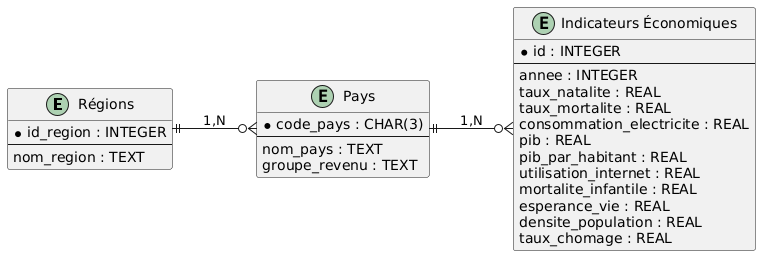
\includegraphics[scale=0.5]{Images/MCD.png}
    \caption{Modèle Conceptuel de Données (MCD)}
    \label{fig:mcd}
\end{figure}

La figure~\ref{fig:mcd} illustre le MCD. On y voit les entités \texttt{Region}, \texttt{Pays}, \texttt{Indicateur}, et \texttt{IndiceDeveloppement}, ainsi que leurs relations. Par exemple, la relation \texttt{APPARTIENT} relie une région à plusieurs pays, tandis que les relations \texttt{MESURE} et \texttt{CALCULE} relient un pays à ses indicateurs et indices de développement respectivement.

\subsubsection*{Modèle Logique de Données (MLD)}

Le MLD est une traduction du MCD en un modèle adapté à une base de données relationnelle. Il définit les tables, leurs colonnes, et les relations entre elles. Voici les principales tables du MLD :

\begin{itemize}
  \item \textbf{Table \texttt{regions}} : Contient les colonnes \texttt{id\_region} (clé primaire) et \texttt{nom\_region}.
  \item \textbf{Table \texttt{pays}} : Contient les colonnes \texttt{code\_pays} (clé primaire), \texttt{nom\_pays}, \texttt{id\_region} (clé étrangère vers \texttt{regions}), et \texttt{groupe\_revenu}.
  \item \textbf{Table \texttt{indicateurs}} : Contient les colonnes \texttt{id} (clé primaire), \texttt{code\_pays} (clé étrangère vers \texttt{pays}), \texttt{annee}, et divers indicateurs économiques comme \texttt{pib}, \texttt{esperance\_vie}, ou \texttt{taux\_chomage}.
  \item \textbf{Table \texttt{indices\_dvpt}} : Contient les colonnes \texttt{id} (clé primaire), \texttt{code\_pays} (clé étrangère vers \texttt{pays}), \texttt{annee}, et des indices de développement comme \texttt{idh}, \texttt{emissions\_co2}, ou \texttt{inegalite\_education}.
\end{itemize}

\begin{figure}[H]
    \centering
    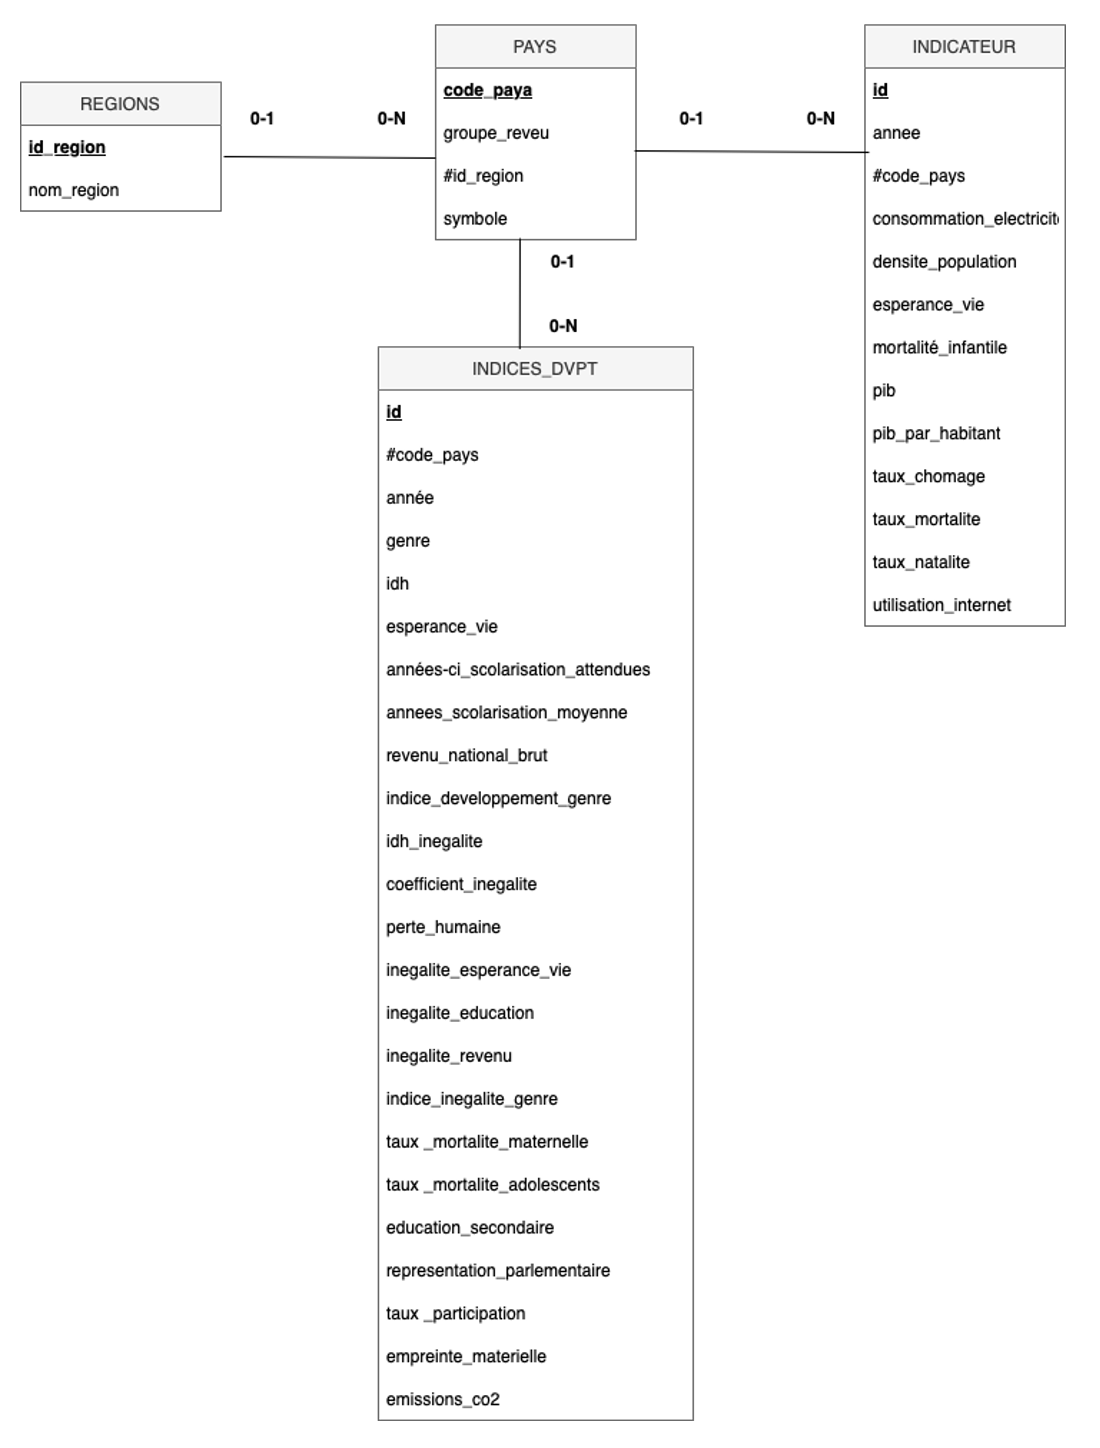
\includegraphics[scale=0.5]{Images/MLD.png}
    \caption{Modèle Logique de Données (MLD)}
    \label{fig:mld}
\end{figure}

La figure~\ref{fig:mld} montre le MLD, où les entités du MCD sont traduites en tables relationnelles. Les relations sont implémentées à l'aide de clés primaires et de clés étrangères. Par exemple, la colonne \texttt{id\_region} dans la table \texttt{pays} est une clé étrangère pointant vers la table \texttt{regions}, et la colonne \texttt{code\_pays} dans les tables \texttt{indicateurs} et \texttt{indices\_dvpt} est une clé étrangère pointant vers la table \texttt{pays}.

\subsubsection*{Conclusion}

Le MCD et le MLD jouent un rôle fondamental dans la conception de la base de données de ce projet. Le MCD fournit une vue d'ensemble des données et de leurs relations, tandis que le MLD traduit cette vue en une structure exploitable par un système de gestion de base de données relationnelle. Ces modèles garantissent une organisation claire et cohérente des données, facilitant ainsi leur exploitation dans le tableau de bord interactif.

\subsection{Conception de la visualisation}

L’outil a été développé en utilisant Chart.js pour l'intégralité des graphiques, à l'exception de la carte interactive sur le dashboard, réalisée par Romain avec D3.js. Ces technologies ont permis de créer des visualisations dynamiques et interactives adaptées aux besoins du projet.

Pour garantir une organisation claire et modulaire, nous avons respecté la structure MVC (Modèle-Vue-Contrôleur) tout au long du développement. Voici une explication détaillée de cette structure et de son application dans le projet :

\begin{itemize}
  \item \textbf{Modèle (Model)} : Le modèle est responsable de la gestion des données. Dans notre projet, les modèles sont implémentés dans les fichiers situés dans le dossier \texttt{/models/}. Ces fichiers interagissent directement avec la base de données MySQL pour récupérer, insérer ou mettre à jour les données. Par exemple, les données des indicateurs économiques ou des régions sont récupérées via des requêtes SQL dans les modèles, puis renvoyées sous forme de tableaux associatifs.

  \item \textbf{Vue (View)} : La vue est chargée de l'affichage des données. Dans notre projet, les fichiers situés dans le dossier \texttt{/views/} contiennent le code HTML et JavaScript nécessaire pour afficher les graphiques et la carte interactive. Par exemple, les graphiques générés avec Chart.js et la carte interactive réalisée avec D3.js sont intégrés dans les fichiers de vue. Ces fichiers reçoivent les données du contrôleur et les affichent de manière visuelle et interactive.

  \item \textbf{Contrôleur (Controller)} : Le contrôleur agit comme un intermédiaire entre le modèle et la vue. Les fichiers situés dans le dossier \texttt{/controllers/} reçoivent les requêtes des utilisateurs (par exemple, via des actions spécifiques dans l'URL), appellent les modèles pour récupérer les données nécessaires, et transmettent ces données aux vues. Par exemple, le fichier \texttt{indicateurs.php} dans \texttt{/controllers/} gère les requêtes pour récupérer les données des indicateurs et les renvoie sous forme de JSON pour être utilisées dans les graphiques.
\end{itemize}

\newpage
Cette structure MVC a permis de séparer clairement les responsabilités, rendant le code plus lisible, modulaire et maintenable. Voici un exemple concret de son fonctionnement dans le cadre de la visualisation des données :
\begin{enumerate}
  \item Lorsqu'un utilisateur sélectionne un indicateur et une année sur l'interface, une requête est envoyée au contrôleur (\texttt{indicateurs.php}) via une URL spécifique.
  \item Le contrôleur appelle le modèle correspondant (par exemple, \texttt{indicateur.php}) pour récupérer les données nécessaires depuis la base de données.
  \item Les données récupérées sont renvoyées au contrôleur, qui les formate en JSON et les transmet à la vue.
  \item La vue utilise ces données pour générer un graphique interactif avec Chart.js ou mettre à jour la carte interactive avec D3.js.
\end{enumerate}

\begin{figure}[H]
    \centering
    \includegraphics[scale=0.35]{Images/figure2.png}
    \caption{Architecture du tableau de bord interactif, intégrant Chart.js et D3.js dans une structure MVC}
\end{figure}

La figure ci-dessus illustre l'architecture du tableau de bord interactif, où chaque composant (modèle, vue, contrôleur) joue un rôle spécifique pour garantir une expérience utilisateur fluide et une gestion efficace des données.

%%%%%%%%%%%%%%%%%
\pagebreak
%%%%%%%%%%%%%%%%%

\section*{\begin{center} \Huge Livrable du projet \end{center}}
\addcontentsline{toc}{section}{\Large Livrable du projet \vspace{0.3cm}}

Le livrable final est un tableau de bord interactif composé de trois pages principales :

\begin{itemize}
  \item \textbf{Page des informations par pays} :
    \begin{itemize}
      \item Permet de sélectionner un pays, une année, et un indicateur.
      \item Affiche un tableau descriptif des différentes valeurs disponibles pour le pays et l'année sélectionnés.
      \item Affiche un graphique montrant l'évolution des données depuis l'année sélectionnée jusqu'à la plus récente dans la base de données pour le pays et l'indicateur choisis.
    \end{itemize}
\vspace{1cm}
    \begin{figure}[H]
        \centering
        \includegraphics[scale=0.5]{Images/info_pays.png}
        \caption{Page des informations par pays : tableau descriptif et graphique d'évolution}
        \label{fig:info_pays}
    \end{figure}

\newpage
  \item \textbf{Dashboard principal} :
    \begin{itemize}
      \item Présente quatre graphiques interactifs affichant différents indicateurs économiques.
      \item Inclut une carte interactive permettant de changer l'année et l'indicateur affichés sur la carte.
      \item Permet une visualisation globale des données économiques à travers des graphiques et une carte.
    \end{itemize}
\vspace{1cm}
    \begin{figure}[H]
        \centering
        \includegraphics[scale=0.4]{Images/figure2.png}
        \caption{Page du dashboard : Graphique Chart.js et Map interactive avec D3.js}
        \label{fig:dashboard}
    \end{figure}
    
\newpage

  \item \textbf{Page de comparaison entre pays} :
    \begin{itemize}
      \item Permet de sélectionner deux pays et un indicateur.
      \item Affiche deux indicateurs pertinents pour chaque pays sous forme de KPI (Key Performance Indicators) côte à côte.
      \item Affiche un graphique comparatif montrant les données associées aux deux pays pour l'indicateur sélectionné.
    \end{itemize}
\vspace{1cm}
    \begin{figure}[H]
        \centering
        \includegraphics[scale=0.5]{Images/comparaison_pays.png}
        \caption{Page de comparaison entre pays : KPI et graphique comparatif}
        \label{fig:comparaison_pays}
    \end{figure}
\end{itemize}

%%%%%%%%%%%%%%%%%
\pagebreak
%%%%%%%%%%%%%%%%%

\section*{\begin{center} \Huge Contributions individuelles \end{center}}
\addcontentsline{toc}{section}{\Large Contributions individuelles \vspace{0.3cm}}

\subsection*{Anthony YON}
\subsubsection*{Tâches réalisées}
Premièrement, dans la partie Backend, je me suis occupé de réaliser la connexion à la base de données dans \texttt{config.inc.php} (par la suite modifiée et perfectionnée par Romain). Ensuite, j’ai pu réaliser les fonctions du modèle \texttt{pays.php}, qui interroge directement la base de données afin de récupérer des informations sur les pays, comme son nom l’indique. J’ai donc créé les fonctions \texttt{getPays()}, \texttt{getDetailsPays()}, \texttt{getPaysParRegion()}, \texttt{getPaysParGroupeRevenu()}, \texttt{getRegions()} et \texttt{getNombrePaysParRegion()}.

Une fois mes tâches Backend réalisées, j’ai confectionné quelques-unes des actions dans le contrôleur \texttt{indicateurs.php}, qui m’ont servi pour confectionner le dashboard principal \texttt{dashboard.php}. Dans ce dernier, qui sert de page d’accueil de notre application en affichant des visuels concernant des données générales sur les données fournies, j’ai réalisé deux graphiques (``Évolution du PIB mondial par année'' et ``Évolution du ratio natalité/mortalité par région'') qui ont nécessité la mise en place d’un code spécifique dans \texttt{graphiques.js}. J’ai aussi fait le \texttt{header.php} et le \texttt{footer.php}.

J’ai également été chargé de réaliser la page \texttt{comparaison\_pays.php}. L’objectif était de créer une page interactive où l’on peut sélectionner deux pays et un indicateur afin d’afficher un graphique en courbe qui comparera l’indicateur au fil des années pour les deux pays. On retrouvera également sur cette page deux KPI.

\subsubsection*{Difficultés rencontrées}
Je n’ai pas rencontré de difficultés particulières à la réalisation de la connexion à la base de données, excepté le fait de bien utiliser une base de données MySQL comme vu en cours. L’enjeu du modèle \texttt{pays.php}, comme pour les autres modèles, était d’optimiser le nombre de fonctions par rapport à nos besoins et la gestion des erreurs en cas de requête erronée.

C’est pour la partie contrôleur que ça s’est compliqué puisqu’avant de faire quoi que ce soit, il fallait bien avoir en tête l’architecture models-controllers-views. Au début, il a fallu que je refasse un point sur tous nos fichiers et leurs fonctions pour ensuite pouvoir coder sans risque. La gestion des erreurs silencieuses en PHP, notamment dans les requêtes SQL, a été un autre défi important, car la moindre faute de frappe pouvait entraîner des retours vides ou des erreurs JSON que j’ai pu détecter avec les fichiers tests ou dans la console. Il a aussi fallu bien structurer les réponses JSON pour qu’elles soient compatibles avec les appels JavaScript, notamment pour les graphiques ou les comparaisons entre pays.

Dans la partie Frontend, pour \texttt{dashboard.php}, la principale difficulté était de réussir à créer un visuel moderne et harmonieux qui donnerait envie à l’utilisateur de rester sur notre application. C’était globalement les mêmes défis pour \texttt{comparaison\_pays.php}, en rajoutant la dimension interactive qu’il a fallu gérer dans \texttt{interactions.js}.

\subsubsection*{Méthodologie}
Pour \texttt{pays.php}, j’ai commencé par tester les requêtes SQL dans phpMyAdmin. Une fois vérifiées, j’ai pu commencer à écrire mes fonctions en utilisant des requêtes paramétrées. L’utilisation de \texttt{mysqli\_prepare()} m’a permis de rendre la requête plus sécurisée et performante. Par exemple, au final, la fonction \texttt{getPaysParGroupeRevenu()} prend en paramètres le groupe de revenu et retourne la liste des pays sous forme de tableaux associatifs.

Pour \texttt{indicateurs.php}, son but est de faire le lien entre les modèles et les vues en jouant le rôle d’interface API : il centralise les appels aux différentes fonctions du Backend en fonction de ce dont nous avons besoin dans le Frontend, récupère les données traitées dans les modèles puis les renvoie au format JSON afin qu’elles puissent être exploitées dans le \texttt{dashboard.php}, etc.

Pour \texttt{header.php} et \texttt{footer.php}, j’ai simplement capitalisé mes connaissances en HTML et CSS pour, avec des classes et des identifiants, formater le bandeau correspondant.

Pour réaliser mes deux graphiques dans \texttt{dashboard.php}, j’ai utilisé Chart.js dans \texttt{graphiques.js}, comme vu en cours, avec le bloc de données, le bloc de configuration et le bloc d’affichage, tout cela renseigné dans une fonction pour l’utiliser dans le visuel final. Pour que cela fonctionne, il était primordial que mon contrôleur renvoie les données au format JSON.

Pour \texttt{comparaison\_pays.php}, une partie de la méthodologie est la même que pour \texttt{dashboard.php}, à la différence près qu’ici j’avais à créer un formulaire HTML et notamment des listes déroulantes \texttt{Pays1} et \texttt{Pays2} avec les données récupérées par les requêtes dans le modèle \texttt{pays.php}. L’utilisation de \texttt{interactions.js} et \texttt{graphiques.js} a été requise pour que le graphique et les KPI s’adaptent bien aux pays sélectionnés.

\subsubsection*{Conclusion}
Ce projet m’a permis de mettre en pratique de façon concrète l’architecture MVC et d’approfondir mes compétences aussi bien en PHP Backend qu’en JavaScript Frontend. J’ai particulièrement apprécié le travail d’interconnexion entre les modèles, le contrôleur et les vues, qui m’a permis de mieux comprendre les enjeux d’une application web dynamique. Ce fut un excellent exercice de rigueur, de logique et de collaboration, notamment pour assurer la cohérence des données du Backend jusqu’à leur affichage côté client. J’ai également apprécié le travail en groupe et notamment avec Romain, qui a su écouter et comprendre les problèmes que j’ai pu rencontrer pendant tout ce projet et m’accompagner dans la résolution de ces derniers.

\subsection*{Mandir DIOP}
\subsubsection*{Tâches réalisées}
\begin{itemize}

    \vspace{0.2cm}
    
    \item Création et maintien du code dans \texttt{config.inc.php}.

    \vspace{0.2cm}
    
    J'ai développé le fichier de configuration pour gérer la connexion à la base de données SQLite en utilisant le pattern Singleton, permettant une connexion unique et optimisée tout au long de l'exécution du script.

    \vspace{0.2cm}
    
    Cependant, ce code nécessite une adaptation selon le système d’exploitation utilisé (Mac ou Windows). Sous macOS, une authentification par mot de passe est requise pour se connecter à la base de données via phpMyAdmin avec MAMP.

    \vspace{0.2cm}
    
    \item Création et maintien du code dans \texttt{/models/indicateur.php}. 
    
    \vspace{0.2cm}
    
    Ce modèle assure l’interaction avec la base de données pour récupérer les informations sur les indicateurs concernant chaque pays. 

    \vspace{0.2cm}
    
    Ce fichier contient notamment les fonctions : 
    
    \vspace{0.05cm}
    
\begin{itemize}
    \item \texttt{getIndicateurs()}
    \item \texttt{getValeursIndicateur()}
    \item \texttt{getMoyenneIndicateurParRegion()}
    \item \texttt{getIndicateursParAnnee()}
    \item \texttt{getIndicateursParAnneePays()}
\end{itemize}
    
    \vspace{0.2cm}
    
    Ces fonctions permettent respectivement de récupérer dynamiquement la liste des indicateurs disponibles, les valeurs d’un indicateur pour un pays donné, la moyenne d’un indicateur par région, l’ensemble des indicateurs pour une année spécifique, ainsi que les données pour un pays et une année donnés. Ces fonctions facilitent l’accès et le traitement des données stockées dans la base pour les afficher sur l’interface web.

    \vspace{0.2cm}
    
    \item \textbf{Création du MLD (Modèle Logique de Données)}.
    
    \vspace{0.2cm}

    
    
Quatre tables principales ont été conçues : \texttt{REGIONS}, \texttt{PAYS}, \texttt{INDICATEUR} et \texttt{INDICES\_DVPT}, avec des relations de type 1-N pour représenter les données économiques par pays et par année.

\subsection*{1. Table \texttt{REGIONS}}
La table \texttt{REGIONS} contient les identifiants et noms des grandes régions. \\
\textbf{Clé primaire} : \texttt{id\_region} \\
\textbf{Relation} : Une région peut contenir plusieurs pays (relation 1-N). Sa clé primaire est utilisée comme clé étrangère dans la table \texttt{PAYS} (\texttt{\#id\_region}).

\subsection*{2. Table \texttt{PAYS}}
Cette table contient les pays ainsi que leur appartenance régionale et leur groupe de revenu. \\
\textbf{Clé primaire} : \texttt{code\_pays} \\
\textbf{Relations} :
\begin{itemize}
  \item \texttt{code\_pays} est référencée comme clé étrangère dans \texttt{INDICES\_DVPT} et \texttt{INDICATEUR}.
  \item \texttt{\#id\_region} est une clé étrangère vers \texttt{REGIONS(id\_region)}.
\end{itemize}

\subsection*{3. Table \texttt{INDICES\_DVPT}}
Cette table contient des indicateurs de développement humain (IDH, espérance de vie, inégalités, etc.) par pays et par année. \\
\textbf{Clé primaire} : \texttt{id} \\
\textbf{Clé étrangère} : \texttt{\#code\_pays} référence la table \texttt{PAYS(code\_pays)}.

\subsection*{4. Table \texttt{INDICATEUR}}
Elle stocke d'autres indicateurs économiques (PIB, taux de chômage, etc.). \\
\textbf{Clé primaire} : \texttt{id} \\
\textbf{Clé étrangère} : \texttt{\#code\_pays} référence également \texttt{PAYS(code\_pays)}.

\vspace{1cm}
\section*{Résumé des relations entre les tables}

\begin{center}
\begin{tabular}{>{\ttfamily}l >{\ttfamily}l >{\ttfamily}l l}
\toprule
\textbf{Clé source} & \textbf{Table cible} & \textbf{Champ cible} & \textbf{Type de relation} \\
\midrule
id\_region          & PAYS                & \#id\_region          & 1 région → N pays \\
code\_pays          & INDICES\_DVPT       & \#code\_pays          & 1 pays → N indices développement \\
code\_pays          & INDICATEUR          & \#code\_pays          & 1 pays → N indicateurs économiques \\
\bottomrule
\end{tabular}
\end{center}

 \vspace{0.2cm}
    
    \item Création et maintien du code dans \texttt{/views/infos\_pays.php}.

    \vspace{0.2cm}
    
    Ce code crée une interface web interactive (informations sur les pays) permettant de sélectionner un pays, une année et un indicateur économique.
    Il affiche les informations générales du pays, sa région et un tableau regroupant plusieurs indicateurs (PIB, espérance de vie, etc.) de l'année choisie.
    \vspace{0.2cm}
    
    Un graphique (via Chart.js) qui illustre l’évolution d’un indicateur sélectionné en l'année choisie et 2018.
    \vspace{0.2cm}
    
    Le tout est mis à jour dynamiquement grâce à un script JavaScript (interaction\_info.js).
    Cette vue permet une exploration simple et visuelle des données par pays et par année.
    \vspace{0.2cm}
        
    \item Création et maintien du code dans \texttt{/controllers/indicateur.php} concernant \newline \texttt{/views/infos\_pays.php}. 
    
        \vspace{0.2cm}
        
        Le contrôleur gère la logique de récupération des données à l’aide des fonctions définies dans \texttt{/models/inndicateur.php}, selon l’action demandée : \vspace{0.2cm} 
        \item (par exemple ?action=getMoyennePIBMondial), il renvoie les résultats sous forme de JSON.
    Ce fichier permet d'aliment dynamiquement les graphiques sur la page infos\_pays.php
    
    \vspace{0.2cm}
    
    \item Création du graphique en barre empilés (Top 5 des pays avec les grand PIB par régions) sur le dashboard principal. Ce graphique en barres empilées présente les 5 pays ayant le plus grand PIB dans chaque région. Les barres sont regroupées par région et chaque segment représente un pays avec sa contribution au PIB régional. 

\end{itemize}

\subsubsection*{Difficultés rencontrées}
\begin{itemize}
    \item Gestion des valeurs manquantes dans la base de données (un nombre considérable de valeur manquantes concernant surtout les indicateurs).
    \item Optimisation de requêtes SQL pour la récupération et extractions des données.
    \item Adaptation du format des données à Chart.js.
    \item Maintien de la cohérence et de l’intuitivité de l’interface utilisateur en se basant sur les choix d'affichage.
    \item  Rendre la page interactivte
\end{itemize}

\subsubsection*{Méthodologie}
\begin{itemize}
    \item \textbf{Analyse préliminaire} : étude de la structure de la base de données et identification des relations clés entre les différentes tables.
    \item \textbf{Conception du MLD} : modélisation des entités, des attributs et des relations, avec une séparation claire des responsabilités pour faciliter l’implémentation.
    \item \textbf{Sécurisation} : usage de requêtes paramétrées, validation systématique des entrées utilisateur, et prévention contre les injections SQL.

\subsection*{Courteney SAINT-HUBERT}
\subsubsection*{Tâches réalisées}
\subsubsection*{Difficultés rencontrées}
\subsubsection*{Méthodologie}
\subsubsection*{Conclusion}

\newpage
\subsection*{Romain LESUEUR}
\subsubsection*{Tâches réalisées}
Premièrement, j’ai créé et maintenu le code dans \texttt{/models/data.php}, ainsi que le dossier \texttt{/tests/} et le logger. J’ai également assisté au développement des parties \texttt{/views/} et \texttt{/controllers/}. J’ai conçu et maintenu le code dans \texttt{/controllers/indicateurs.php} pour le dashboard principal. En parallèle, j’ai rédigé et maintenu les fichiers \texttt{DEV.md}, \texttt{README.md}, \texttt{.htaccess}, et \texttt{/docs/howtogit.md}. J’ai aussi réalisé au moins un graphique sur le dashboard principal et supervisé l’ensemble du projet.

En tant que superviseur, j’ai également coordonné les tâches entre les membres de l’équipe, en m’assurant que chacun comprenne ses responsabilités et puisse avancer efficacement. J’ai pris en charge la validation des contributions, en effectuant des revues de code régulières pour garantir la qualité et la cohérence du projet. J’ai également fourni des exemples concrets pour guider mes coéquipiers, notamment en développant des fonctions et des graphiques de référence.

\subsubsection*{Difficultés rencontrées}
La principale difficulté a été de travailler avec des personnes qui n’avançaient pas au même rythme ni au même niveau. Cela a nécessité une grande adaptabilité et une communication constante pour maintenir une dynamique de groupe positive. L’interdiction d’utiliser la POO a également été un défi, car cela limitait certaines optimisations et structurations du code. Enfin, l’exploration de D3.js pour la carte interactive a représenté un apprentissage important, car je n’avais jamais utilisé cette technologie auparavant.

Un autre défi a été de gérer les imprévus liés aux retards de certains membres, ce qui m’a poussé à reprendre certaines parties du projet pour respecter les délais. Cela a parfois créé une surcharge de travail, mais cela m’a également permis de renforcer mes compétences en gestion de projet et en résolution de problèmes.

\subsubsection*{Méthodologie}
Pour ce projet, j’ai essayé de prévoir l’intégralité des fonctions nécessaires dans les modèles. J’ai rédigé le guide de développement et le \texttt{README.md} avant même de commencer à coder. Cependant, certaines fonctions dans les modèles ne sont pas utilisées, et d’autres ne sont pas mentionnées, ce qui reflète une planification initiale encore floue. J’ai décidé de développer d’abord les modèles, puis les vues, et enfin le contrôleur. Avec du recul, commencer par définir les vues aurait permis d’avoir une idée plus claire des besoins côté modèles.

J’ai donné ma vision pour chaque vue à développer, car certains membres étaient un peu perdus au début. Bien que je ne souhaitais pas imposer ma vision, elle a finalement été conservée. J’ai développé tous les tests et imposé une sortie uniforme sous forme de tableau associatif pour toutes les fonctions, afin de simplifier leur traitement dans les contrôleurs.

Les tests avaient pour but principal de fournir des exemples types et de visualiser les sorties via des pages de test accessibles sur le localhost (par exemple, localhost/DED/tests/test\_indicateur.php). Concernant le dashboard, j’ai développé une fonction pour générer un graphique simple (évolution de l’espérance de vie), qui a servi d’exemple pour Anthony et Mandir dans leurs propres graphiques.

J’ai également réalisé une carte interactive avec D3.js, bien que Chart.js ait été imposé. Mon objectif était de reproduire une fonctionnalité vue dans une démo de l’entreprise Digdash, spécialisée en Business Intelligence. Cette carte permet une exploration approfondie des données. Cependant, des limitations sont apparues, notamment liées à la correspondance entre les fichiers GeoJSON et notre base de données. Par exemple, le Soudan du Sud n’apparaît pas dans la vue continentale mais est visible dans la vue régionale. Malgré ces imperfections, cette carte a été bien accueillie, notamment par le RH de Digdash, ce qui m’a permis d’obtenir un stage chez eux.

Enfin, j’ai retouché le travail de chaque membre du groupe, non pas pour effacer leur contribution, mais pour leur montrer comment aller plus loin dans leur raisonnement. J’ai également pris le temps de documenter les parties critiques du projet pour faciliter leur compréhension et leur maintenance future.

\subsubsection*{Conclusion}
J’ai grandement apprécié travailler avec Anthony, qui a été une belle surprise cette année. Ce projet m’a permis de travailler sur mon adaptabilité et de m’imposer comme chef de projet, ce qui m’a fait progresser en gestion de projet globale. Sur le plan technique, j’ai pu explorer l’utilisation de D3.js, ce qui a été une expérience enrichissante. Ce projet m’a également permis de renforcer mes compétences en communication et en leadership, des qualités essentielles pour mener à bien des projets collaboratifs complexes.

%%%%%%%%%%%%%%%%%
\pagebreak
%%%%%%%%%%%%%%%%%

\section*{\begin{center} \Huge Conclusion globale \end{center}}
\addcontentsline{toc}{section}{\Large Conclusion globale \vspace{0.3cm}}

Ce projet a représenté une opportunité concrète de mettre en œuvre nos compétences techniques au sein d’un travail collaboratif. Malgré les contraintes de temps, les aléas extérieurs et les différences d’investissement entre les membres, nous sommes parvenus à aboutir à un résultat satisfaisant, stable et fonctionnel.  

La répartition du travail s’est révélée inégale au fil des semaines. Certains membres ont dû prendre en charge une part importante du développement, incluant non seulement la création de fonctionnalités mais aussi la correction et l’harmonisation du code produit par d’autres. Ces ajustements, bien qu’invisibles en surface, ont été essentiels pour garantir la cohérence et la qualité globale du projet.  

Anthony a démontré un engagement constant, assurant ses tâches tout en reprenant certaines parties initialement attribuées à d’autres. Il a su concilier ses responsabilités avec son stage, preuve d’un bon sens de l’organisation. Toutefois, il pourrait encore progresser en étant plus proactif et en n’attendant pas systématiquement les validations ou les consignes pour avancer.  

Mandir a connu un démarrage difficile, pénalisé par des problèmes techniques et la charge de son propre stage. Néanmoins, il a su se mobiliser dans la seconde partie du projet, remplissant les tâches qui lui étaient confiées avec un accompagnement ponctuel. Pour les projets futurs, un renforcement de son autonomie et de sa communication serait bénéfique.  

Enfin, la contribution de Courteney est malheureusement restée très limitée pour ne pas dire inexistante. Avec seulement 22 lignes de code inutilisables, son absence d’implication a eu un impact direct sur l’organisation collective. Ce manque de fiabilité a contraint les autres membres à compenser, ce qui a pesé sur la charge de travail globale.

Par ailleurs, le respect du calendrier initial n’a pas pu être assuré. La simultanéité avec d’autres projets à rendre, ainsi que les débuts de stage de certains membres, ont engendré des retards. Toutefois, grâce à une mobilisation progressive et à une bonne coordination en fin de parcours, nous avons su mener ce projet à son terme.

Nous avons également fait le choix de ne pas suivre aveuglément les instructions du projet. Bien que le but principal soit de nous évaluer sur nos capacités techniques, nous avons estimé que le sujet proposé était trop codifié et limitait l'aspect créatif. Par exemple, après avoir discuté avec Matthias et observé son livrable, j'ai constaté qu'il avait une page distincte pour chaque partie correspondant aux sections A, B, C et D. Cependant, nous avons choisi de combiner les parties A et B par exemple, car cela nous semblait plus logique et fluide. Je pense qu'il serait bénéfique que les sujets soient formulés de manière plus floue (sauf pour la stack technique), afin de pousser les étudiants à réfléchir davantage à la manière d'implémenter chaque partie selon leur propre approche. Cela encouragerait une plus grande diversité dans les livrables et stimulerait la créativité.

En somme, au-delà des compétences techniques mobilisées, ce projet a mis en lumière les enjeux humains d’un travail en équipe : l’importance de l’implication individuelle, la nécessité de la communication continue, et la gestion des imprévus. Il s’agit d’une expérience formatrice, riche en enseignements, qui nous permettra d’aborder nos futurs projets avec davantage de rigueur, de coordination et de maturité.

%%%%%%%%%%%%%%%%%
\pagebreak
%%%%%%%%%%%%%%%%%

\addcontentsline{toc}{section}{\listfigurename}
\listoffigures

\end{document}
